\chapter{Problem Definition}
\label{chap2}
\section{Domain}
There are many subdomains under the general unshredding umbrella. Some of the more common distinctions look at how the paper was shredded (eg: strip-cut, cross-cut or hand torn), at the nature of the shredded document (eg: black and white or coloured; text document, picture or mixed) and at the reconstruction method (eg: fully automatic, integrated human expert or crowdsourced). 

Nowadays, most documents are mechanically shredded rather than hand torn, so we decide to focus solely on the strip-cut and the cross-cut variants. Additionally, the most commonly shredded documents are black and white, typed, text documents, so this is the variant we are interested in. Finally, we only look at fully automatic solutions, partly because previous work \cite{P1,P2} has shown that automatic methods can be modified to incorporate user interaction with relative ease.
 
\section{Assumptions}
\label{chap2Ass}
The output of a shredding device, and therefore the input to our algorithm, is a set of $n$ shreds $S = \{s_0, ..., s_{n-1}\}$. The first part of our algorithm is a pre-processing step which aims to transform the real scanned images, containing the shreds, into images we call \emph{ideal shreds}. \\
The ideal shreds have the following properties:
\begin{itemize}
\item Each ideal shred corresponds exactly to a separate image file. That is to say, an ideal shred image file will contain all the pixels belonging to a certain shred and only those pixels.
\item All ideal shreds have the same height and width.
\item All edges on all ideal shreds are either perfectly vertical or perfectly horizontal.
\item All ideal shreds are correctly orientated. That is to say, if the original document were displayed with its longest edge vertically aligned, then all ideal shreds have the same orientation they would have in that original document (note that this means the document may be ``upside down"; this is fine as long as all shreds share the same orientation).
\item The ideal shred image files contain only pure white and pure black pixels.
\end{itemize}

The problem of reducing the real shreds to these ideal shreds is analysed in Chapter \ref{chap6}. For the rest of this work, the input to the algorithm is assumed to consist of ideal shreds (see Figure \ref{fig:idealShreds}).

\begin{figure}[h]
        \setlength{\fboxsep}{-0.1cm}
        \centering
        \fbox{
        \begin{subfigure}[b]{0.079\textwidth}
                \centering
                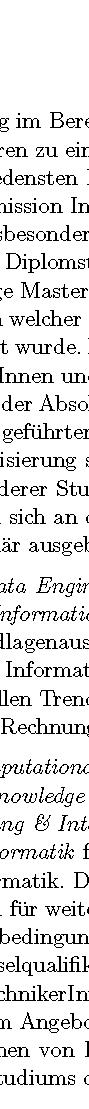
\includegraphics[width=\textwidth]{wip/wip3}
        \end{subfigure}
        }
        ~ 
        \fbox{
        \begin{subfigure}[b]{0.079\textwidth}
                \centering
                
\includegraphics[width=\textwidth]{wip/wip1}
        \end{subfigure}
        } 
        ~ 
        \fbox{
        \begin{subfigure}[b]{0.079\textwidth}
                \centering
                
\includegraphics[width=\textwidth]{wip/wip9}
        \end{subfigure}
        }
        ~ 
        \fbox{
        \begin{subfigure}[b]{0.079\textwidth}
                \centering
                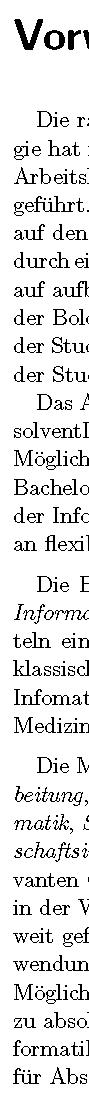
\includegraphics[width=\textwidth]{wip/wip0}
        \end{subfigure}
        } 
        ~ 
        \fbox{ 
        \begin{subfigure}[b]{0.079\textwidth}
                \centering
                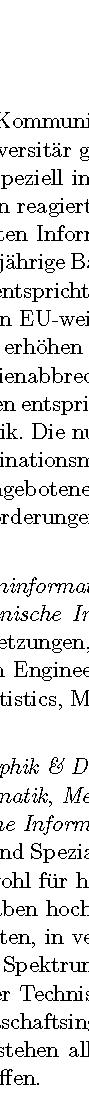
\includegraphics[width=\textwidth]{wip/wip7}
        \end{subfigure}
        } 
        ~ 
        \fbox{ 
        \begin{subfigure}[b]{0.079\textwidth}
                \centering
                
\includegraphics[width=\textwidth]{wip/wip5}
        \end{subfigure}
        } 
        ~ 
        \fbox{ 
        \begin{subfigure}[b]{0.079\textwidth}
                \centering
                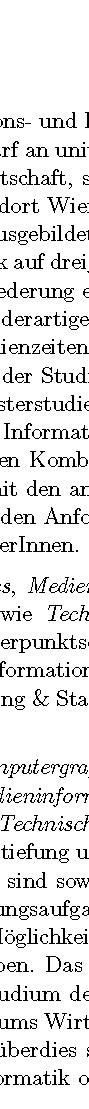
\includegraphics[width=\textwidth]{wip/wip6}
        \end{subfigure}
        } 
        ~ 
        \fbox{
        \begin{subfigure}[b]{0.079\textwidth}
                \centering
                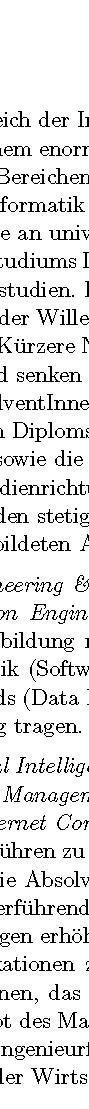
\includegraphics[width=\textwidth]{wip/wip4}
        \end{subfigure}
        } 
        ~ 
        \fbox{ 
        \begin{subfigure}[b]{0.079\textwidth}
                \centering
                
\includegraphics[width=\textwidth]{wip/wip8}
        \end{subfigure}
        } 
        ~ 
        \fbox{ 
        \begin{subfigure}[b]{0.079\textwidth}
                \centering
                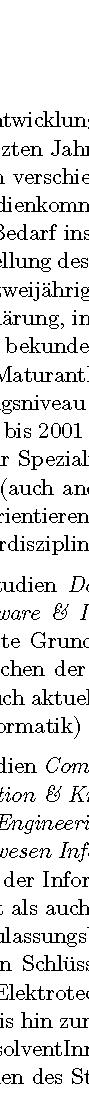
\includegraphics[width=\textwidth]{wip/wip2}
        \end{subfigure}
        }
        \caption{Example of \emph{ideal shreds} of a document. }
        \label{fig:idealShreds}
\end{figure}

Now that we have our ideal shreds, the problem can be further subdivided into two functions.

\section{Formal definition of score and search functions}
\textbf{The edge scoring function:} This first function analyses all pairs of shreds for edge matches and returns a number that represents the quality of each match (see Figure \ref{fig:edgeMatch}).

\begin{figure}[h]
    \centering
    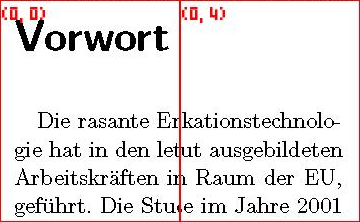
\includegraphics[width=0.8\textwidth]{conf}
    \caption{A potential edge between two shreds. The edge scoring function has to evaluate this match and report how good it is.}
    \label{fig:edgeMatch}
\end{figure}

Formally, we must obtain: $sc_r(s_i, s_j)$ and $sc_b(s_i, s_j), \forall s_i, s_j \in S $ where  $sc_r(s_i, s_j)$ is the score of placing $s_j$ to the right of $s_i$ and $sc_b(s_i, s_j)$ is the score of placing $s_j$ below $s_i$.

\textbf{The global search function:} The second function receives the scores between all pairs of shreds as input and must find an arrangement of shreds in 2D space that optimises the global score.

We consider the global score to be the sum of all individual scores between neighbouring shreds. Modifying the formulation made in \cite{P20}, we can define a solution of the search function as a mapping $ \Pi : D^2 \rightarrow S$ where $D = \{0, ..., |S|-1\}$. This means each position in a two dimensional space defined by $D^2$ corresponds to a shred. Formally
\[
\Pi(r,c) =
\left\{
	\begin{array}{ll}
		\mbox{the shred placed at row r, column c; IF such a shred exists } \\
		\mbox{a completely blank shred; OTHERWISE }
	\end{array}
\right.
, \forall r,c \in D \]

The global score of a shred placement, $GS(\Pi)$ can then be defined as:\footnote{This assumes the shreds are indexed such as $(0,0)$ is the top, leftmost shred and $(|S-1|,|S-1|)$ is the bottom, rightmost shred} \[GS(\Pi) = \sum_{r=1}^{|S|-1} \sum_{c=1}^{|S|-1} (sc_b(\Pi(r-1,c),\Pi(r,c)) + sc_r(\Pi(r,c-1),\Pi(r,c)))  \]
 
\section{Complexity}
The scoring function is forced to calculate a score for each pair of shreds. Therefore, if we have $n$ shreds, we will have to calculate on the order of $n^2$ scores. Looking at the number of pieces that a page can be shred into (Table: \ref{tab:din}), we can see that this quickly becomes a problem. Some techniques that could mitigate this bottleneck are explored in Section \ref{chap3PP}

The search function, on the other hand, has to search the space of all possible two dimensional placements of edges. Since we have no information about the original shape of the document, the space we must consider for $n$ shreds will have $length = height = n$ and therefore $positions = n^2$. This means we are placing $n$ shreds into $n^2$ slots and so the number of possible placements is $\displaystyle {n^2 \choose n} = \frac{n^2!}{n!(n^2-n)!} $. Clearly this is a huge search space and, in fact, \cite{P1} has shown that the search problem is NP-hard even if restricted to just strip-cut documents. Again, looking at Table \ref{tab:din} we can easily see that optimal search solutions are not feasible for this problem and we must therefore make do with heuristics.

\section{Modularity}
By splitting the reconstruction into the three mentioned sub-functions (pre-processing, score and search), we attempt to solve the problem in a modular way.

Any of the three functions could be enhanced, or replaced entirely without needing to make any modifications in the other two functions. This is particularly useful since each function has quite a different goal and utilises different techniques (for instance, all optical character recognition related algorithms will be restricted to the score function). This separation of concerns allows us to improve algorithms more easily or extended them to different problem domains. 

This modularity is something that was aimed at throughout, so that not only can any of the functions be replaced, but they can easily be composed with other functions. These factors will be discussed more thoroughly in the chapters corresponding to each function.
